%TODO: add cliffhanger with preview for next time
%TODO: add learning outcome slide

% Make nice A4 pages for print:
%\usepackage{pgfpages}
%\pgfpagesuselayout{resize to}[a4paper,border shrink=5mm,landscape]

\beamertemplatenavigationsymbolsempty

\setbeamertemplate{bibliography item}[text]

\usepackage[type={CC},modifier={by-sa},version={4.0}]{doclicense}

\usepackage[utf8]{inputenc}
\usepackage{hyperref}
\usepackage{breakurl}
\usepackage{graphicx}
\usepackage{pgfplots}
\usepackage{pgf}
\usepackage{tikz}
\usetikzlibrary{positioning}
\usetikzlibrary{arrows}
\usetikzlibrary{decorations.markings}
\usetikzlibrary{calc}
\usetikzlibrary{matrix}
\usetikzlibrary{shapes}
\usetikzlibrary{decorations.pathmorphing}
\usetikzlibrary{fit}
\usetikzlibrary{backgrounds}
\usetikzlibrary{plotmarks}
\usepackage{stmaryrd}
\usepackage{listings}
\usepackage{pdflscape}
\usepackage{perpage}
\usepackage{appendixnumberbeamer}

%\usepackage[thmmarks,amsmath,amsthm]{ntheorem} % already included in beamer
\usepackage{thm-restate}

\usepackage[sort&compress,numbers]{natbib}  % to be have \citet, \citeauthor, \citeyear

\MakePerPage{footnote}

\tikzstyle{o}=[r,ppBlue]
\tikzstyle{r}=[thick,rectangle,align=center]
\tikzstyle{t}=[r,ppTrans] %,font=\bfseries]
\tikzstyle{dd}=[densely dashed]
\tikzstyle{n}=[r,ppBlue]
\tikzstyle{p}=[r,ppRed]
\tikzstyle{ppRed}  =[draw=red,  fill=  red!20]
\tikzstyle{ppBlue} =[draw=blue, fill= blue!20]
\tikzstyle{ppGreen}=[draw=green,fill=green!20]
\tikzstyle{ppTrans}=[draw=none, fill=none]

\usetheme{Warsaw}

\useoutertheme[subsection=true]{smoothbars}
%\useoutertheme[subsection=false]{miniframes}

\definecolor{bblue}{HTML}{D7DF01}	% yellow-ish actually, for better black/white printing
\definecolor{rred}{HTML}{C0504D}
\definecolor{ggreen}{HTML}{9BBB59}
\definecolor{ppurple}{HTML}{9F4C7C}
\definecolor{lightgray}{rgb}{0.3,0.3,0.3}
\definecolor{lightergray}{rgb}{0.9,0.9,0.9}
\definecolor{UniBlue}{RGB}{83,121,170}

\DeclareTextFontCommand\textintro{\normalfont\bfseries\itshape} % nice!
\newcommand{\intro}[2][]
{%
	\textintro{#2}%
}
\newcommand{\empha}[2][]
{%
	\emph{#2}%
}

%\theoremstyle{plain}
\newcounter{reqcounter}
\newtheorem{requirement}[reqcounter]{Requirement}

%setbeamercolor{structure}{fg=violet}

\makeatletter
\def\th@task{%
    \normalfont % body font
    \setbeamercolor{block title example}{bg=orange,fg=white}
    \setbeamercolor{block body example}{bg=orange!20,fg=black}
    \def\inserttheoremblockenv{exampleblock}
  }
\makeatother

\theoremstyle{task}
\newtheorem{task}{Task}

\newenvironment{assignment}%
{%\setbeamercolor{background canvas}{bg=violet}%
%\setbeamercolor{structure}{fg=cyan!90!black}%
 \setbeamercolor{frametitle}{bg=orange,fg=white}
\begin{frame}}%
{\end{frame}}%

\AtBeginSection[]{
  \begin{frame}
  \vfill
  \centering
  \begin{beamercolorbox}[sep=8pt,center,shadow=true,rounded=true]{title}
    \usebeamerfont{title}\insertsectionhead\par%
  \end{beamercolorbox}
  \tableofcontents
  \vfill
  \end{frame}
}




\pgfplotsset{compat=1.14}
\author{Markus Raab}


\date{25.5.2018}

\begin{document}

\renewcommand{\enquote}[1]{\emph{``#1''}} % Cannot be done earlier

%%%%%%%%%%%%%%%%%%%%%%%%%%%%%%%
\begin{frame}
	\titlepage
	\doclicenseThis
\end{frame}

\begin{frame}
	\frametitle{Organization}
	Schedule:
	\begin{description}
		\item[25.5.2018:] \textbf{team exercise submitted}
		\item[1.6.2018:] lecture
		\item[8.6.2018:] lecture
		\item[15.6.2018:] last corrections of team exercise
		\item[22.6.2018:] oral test
	\end{description}
\end{frame}


\begin{frame}
	\frametitle{Popular Topics}
	\vspace{-0.5cm}
	\begin{multicols}{2}
	\begin{description}
	\item[4] validation
	\item[4] user interface
	\color{red}
	\item[3] tools (benefits?)
	\color{gray}
	\item[3] testability
	\item[3] complexity reduction (when conf. needed?)
	\item[3] architectural decisions
	\color{black}
	\item[2] Puppet
	\color{gray}
	\item[2] modularity
	\item[2] environment variables
	\color{gray}
	\item[2] documentation
	\color{red}
	\item[2] configuration specification
	\color{gray}
	\item[2] command-line args\color{black}
	\color{gray}
	\item[2] code generation
	\item[1] variability
	\color{black}
	\item[1] self-description
	\item[1] round-tripping
	\color{gray}
	\item[1] early detection
	\item[1] introspection
	\item[1] dependences
	\item[1] auto-detection
	\color{red}
	\item[1] context-awareness
	\color{black}
	\item[1] administrators
	\end{description}
	\end{multicols}
\end{frame}

\begin{frame}
	\hspace*{-1cm}\includegraphics[width=\paperwidth]{dot/topics}
\end{frame}

\begin{frame}
	\frametitle{Introspection (Recapitulation)}
	\begin{task}
	What is internal and external specification?
	What is introspection?
	\end{task}

	\pause
	\vspace{1em}

	\begin{itemize}
	\item \textit{internal}: within applications' source code
	\item \textit{introspection}: unified get/set access to (meta*)-key/values
	\item access via applications, CLI, GUI, web-UI, ...
	\item access via any programming language (similar to file systems)
	\item GUI, web-UI can semantically interpret metadata
	\item assemble modular parts (validation, logging, \dots)
	\item needed as communication between producers and consumers
	\item essential for \intro[no-futz computing]{no-futz computing}~\citet{holland2001nofutz}
	\end{itemize}
\end{frame}

\begin{frame}
	\frametitle{Code Generation (Recapitulation)}
	\begin{task}
	Which artifacts can be produced by an code generator?
	\end{task}

	\pause

	\begin{itemize}
	\item documentation (to avoid duplication)
	\item testing (integration, unit, regression, \dots{} tests)
	\item metrics (which configuration settings are used in the source)
	\item examples (e.g., defaults)
	\item auto-completion/syntax highlighting/IDE support
	\item tooling (GUI, Web UI)
	\item validation code
	\item configuration management tool code
	\end{itemize}
\end{frame}

\begin{frame}
	\frametitle{KeySet (Recapitulation)}

	The common data structure of Elektra:
	\vspace{1cm}

	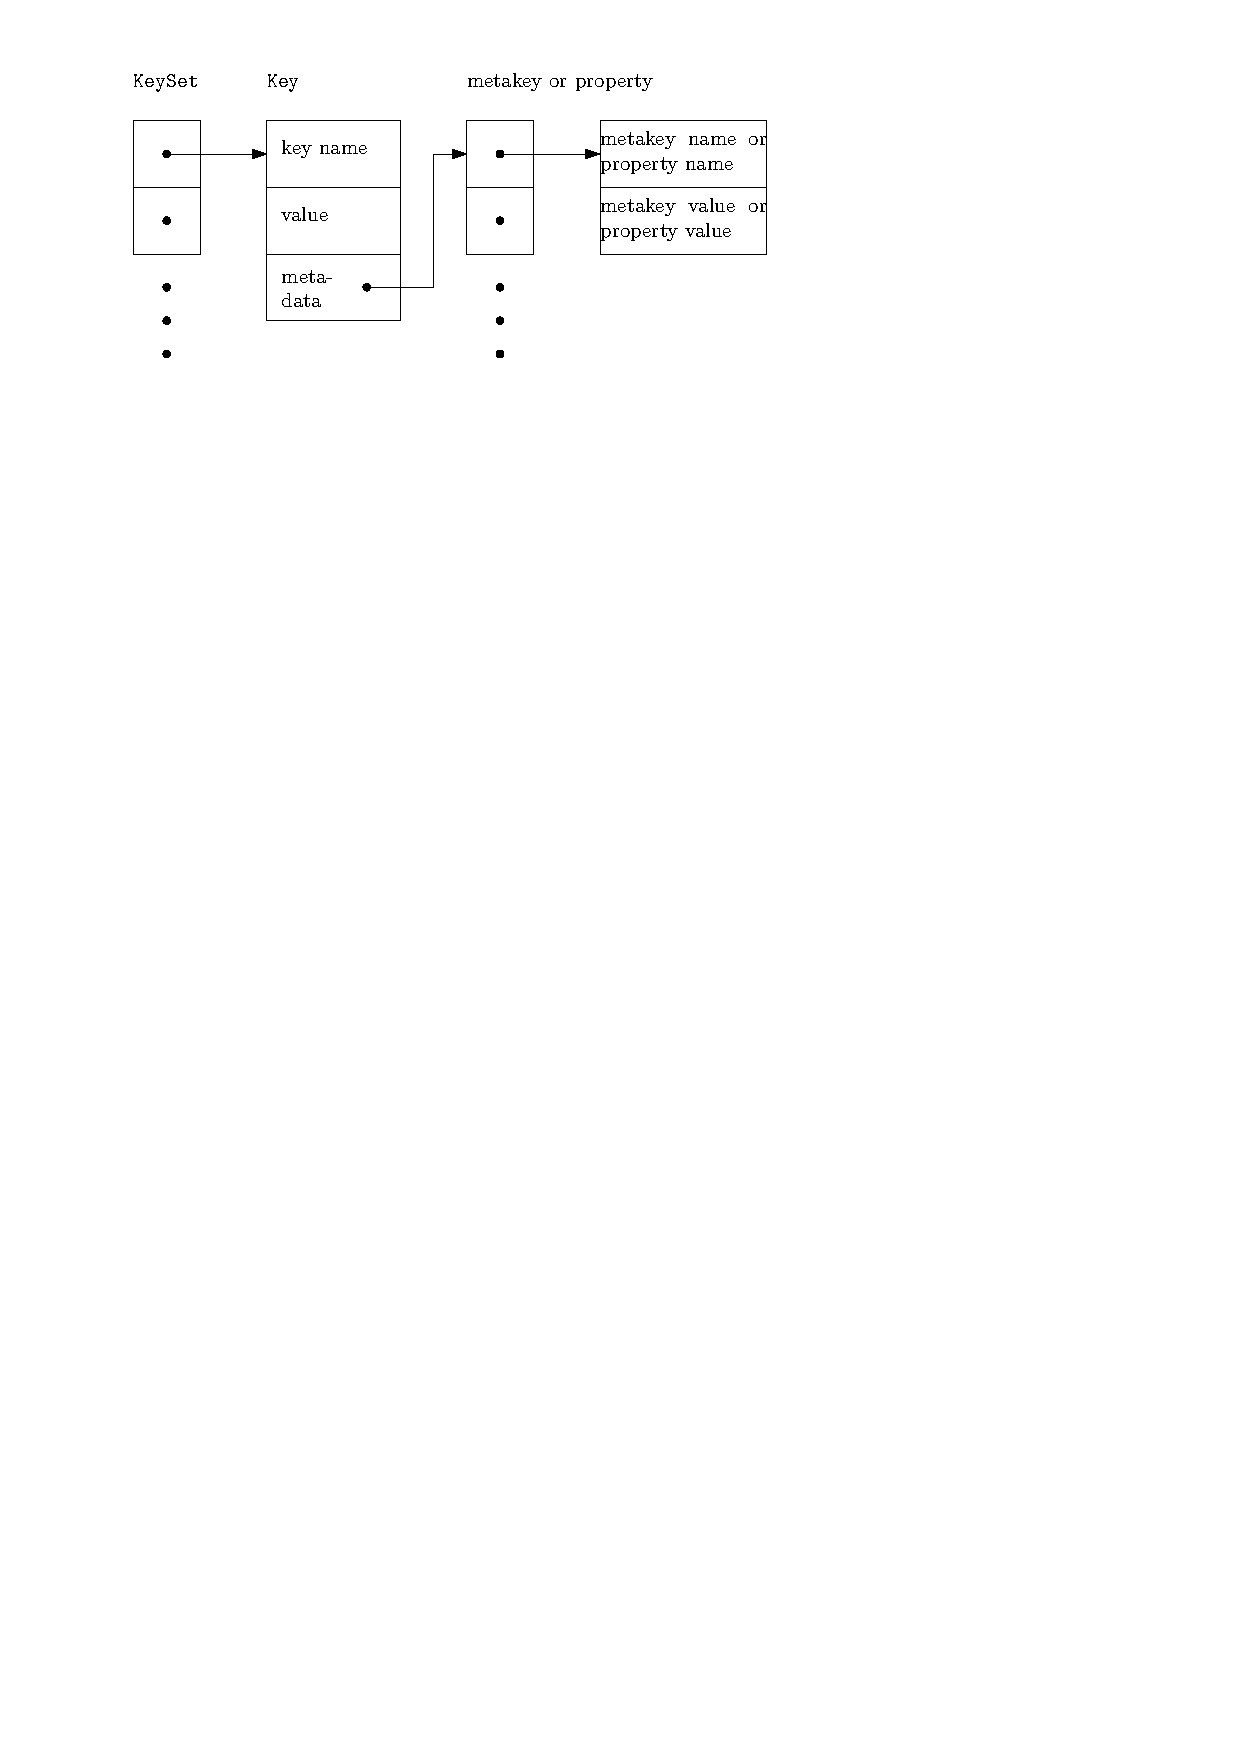
\includegraphics{keyset}
\end{frame}

\begin{frame}
	\frametitle{Testing (Recapitulation)}
	\begin{task}
	What do we want to test?
	\end{task}

	\pause

	\begin{itemize}
	\item That settings do what they should (devs and admins)
	\item That settings are properly validated (devs~\cite{xu2013blame})
	\item Regression tests (devs~\cite{qu2008configuration})
	\vspace{1em}
	\item Are all settings implemented? (devs)
	\item Are all settings used in tests? (devs)
	\item Are there unused settings in the code? (devs)
	\item Do the chosen settings work? (admins)
	\end{itemize}
\end{frame}

\begin{frame}
	\frametitle{Early detection (Recapitulation)}
	\begin{task}
	When do we want to detect misconfiguration?
	\end{task}

	\pause

	Phases when we can detect misconfigurations:
	\begin{itemize} %[<+-| alert@+>]
	\item Compilation stage in configuration management tool
	\item Writing configuration settings on nodes
	\item Starting applications (load-time)
	\item When configuration setting is actually used (run-time)
	\end{itemize}

	\pause[\thebeamerpauses]

	\begin{alertblock}{Problem}
	Earlier versus more context.
	\end{alertblock}
\end{frame}

\begin{frame}[fragile]
	\frametitle{Example Documentation (Recapitulation)}

	\begin{code}[gobble=4]
	[slapd/threads/listener]
	  check/range:=1,2,4,8,16
	  default:=1
	  description:=adjust to use more threads
	  rationale:=needed for many-core systems
	  requirement:=1234
	  visibility:=user
	\end{code}
\end{frame}

\begin{frame}
	\frametitle{Reevaluate specifications (Recapitulation)}

	\begin{task}
	In which situations should you reevaluate if a configuration setting (specification) is needed?
	\end{task}

	\pause

	\ExecuteMetaData[../book/implications.tex]{reasons-adding}

	\begin{alertblock}{Goal}
	Reduction of all not-needed configuration settings (user view).
	\end{alertblock}
\end{frame}


\begin{frame}
	\frametitle{Notification (Recapitulation)}

	\begin{task}
	Why do we need notification?
	\end{task}

	\pause

	\begin{enumerate}
	\item to keep transient and persistent configuration settings always in sync~\cite{jin2014configurations}
	\item to avoid polling of configuration settings
	\item to better integrate into already existing mechanisms (main loops)\footnote{Is one of the main reasons why most framework already integrate configuration settings.}
	\end{enumerate}

	\ExecuteMetaData[../book/motivation.tex]{req-consistency}
\end{frame}

\begin{frame}[fragile]
	\frametitle{Semantic three-way merge (Recapitulation)}

	\textbf{Ours:}
	\begin{code}[gobble=4,language=CfgElektra]
	slapd/threads/listener=4

	slapd/pool/enabled=yes;tried to set no
	\end{code}

	\vspace{1.5em}

	\textbf{Theirs:}
	\begin{code}[gobble=4,language=CfgElektra]
	slapd/pool/enabled=off
	slapd/threads/listener=8
	\end{code}

	\vspace{1.5em}

	\textbf{Origin:}
	\begin{code}[gobble=4,language=CfgElektra]
	slapd/threads/listener=8
	slapd/pool/enabled=on
	\end{code}
\end{frame}

%%%%%%%%%%%%%%%%%%%%%%%%%%%%%%%%%%%%%%%%%% 
\section{Context-Awareness}

\subsection{}

\begin{frame}
	\citet{khalil2005context} conducted a study where all users found context-aware configuration (very) useful.
	They learned that in \p{89} of cases the mapping between activities and settings was consistent for individual users.
	In the study, context-aware configuration improved satisfaction, even if deduced settings sometimes were not appropriate.
	For example, a participant stated:
	\vspace{2em}

	\begin{quote}
	``I like how it changes state without you having to tell it to. I always forget to turn my cell [off] in class and turn it on after.''
	\end{quote}
\end{frame}

\begin{frame}
	\frametitle{Definition (Recapitulation)}
	\ExecuteMetaData[../book/background.tex]{context-definition}
\end{frame}

\begin{frame}
	\frametitle{Types of Configuration (Recapitulation)}
	\begin{description}
	\ExecuteMetaData[../book/background.tex]{context-types}
	\end{description}
\end{frame}

\begin{frame}
	\hspace*{-1em}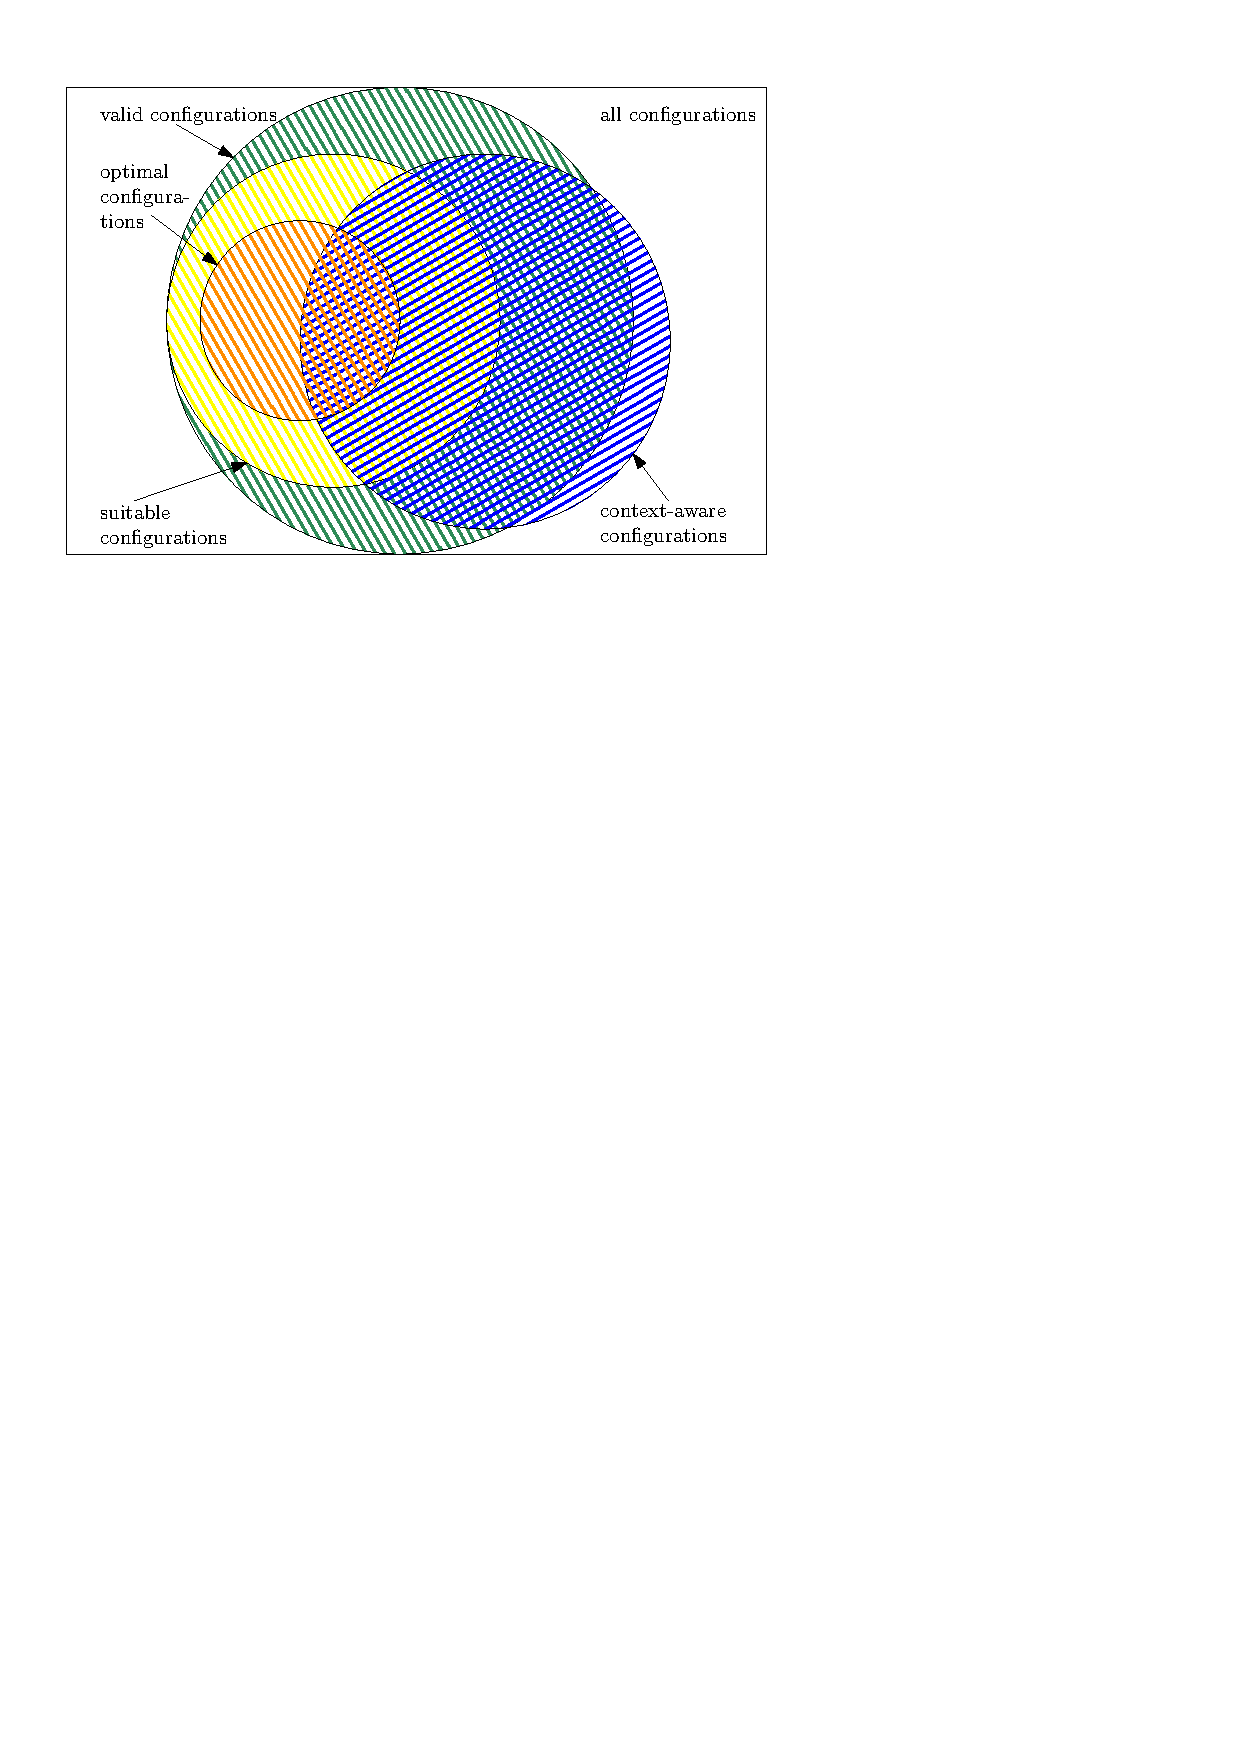
\includegraphics{configurations}
\end{frame}

\begin{frame}
	\frametitle{Cascading (Recapitulation)}
	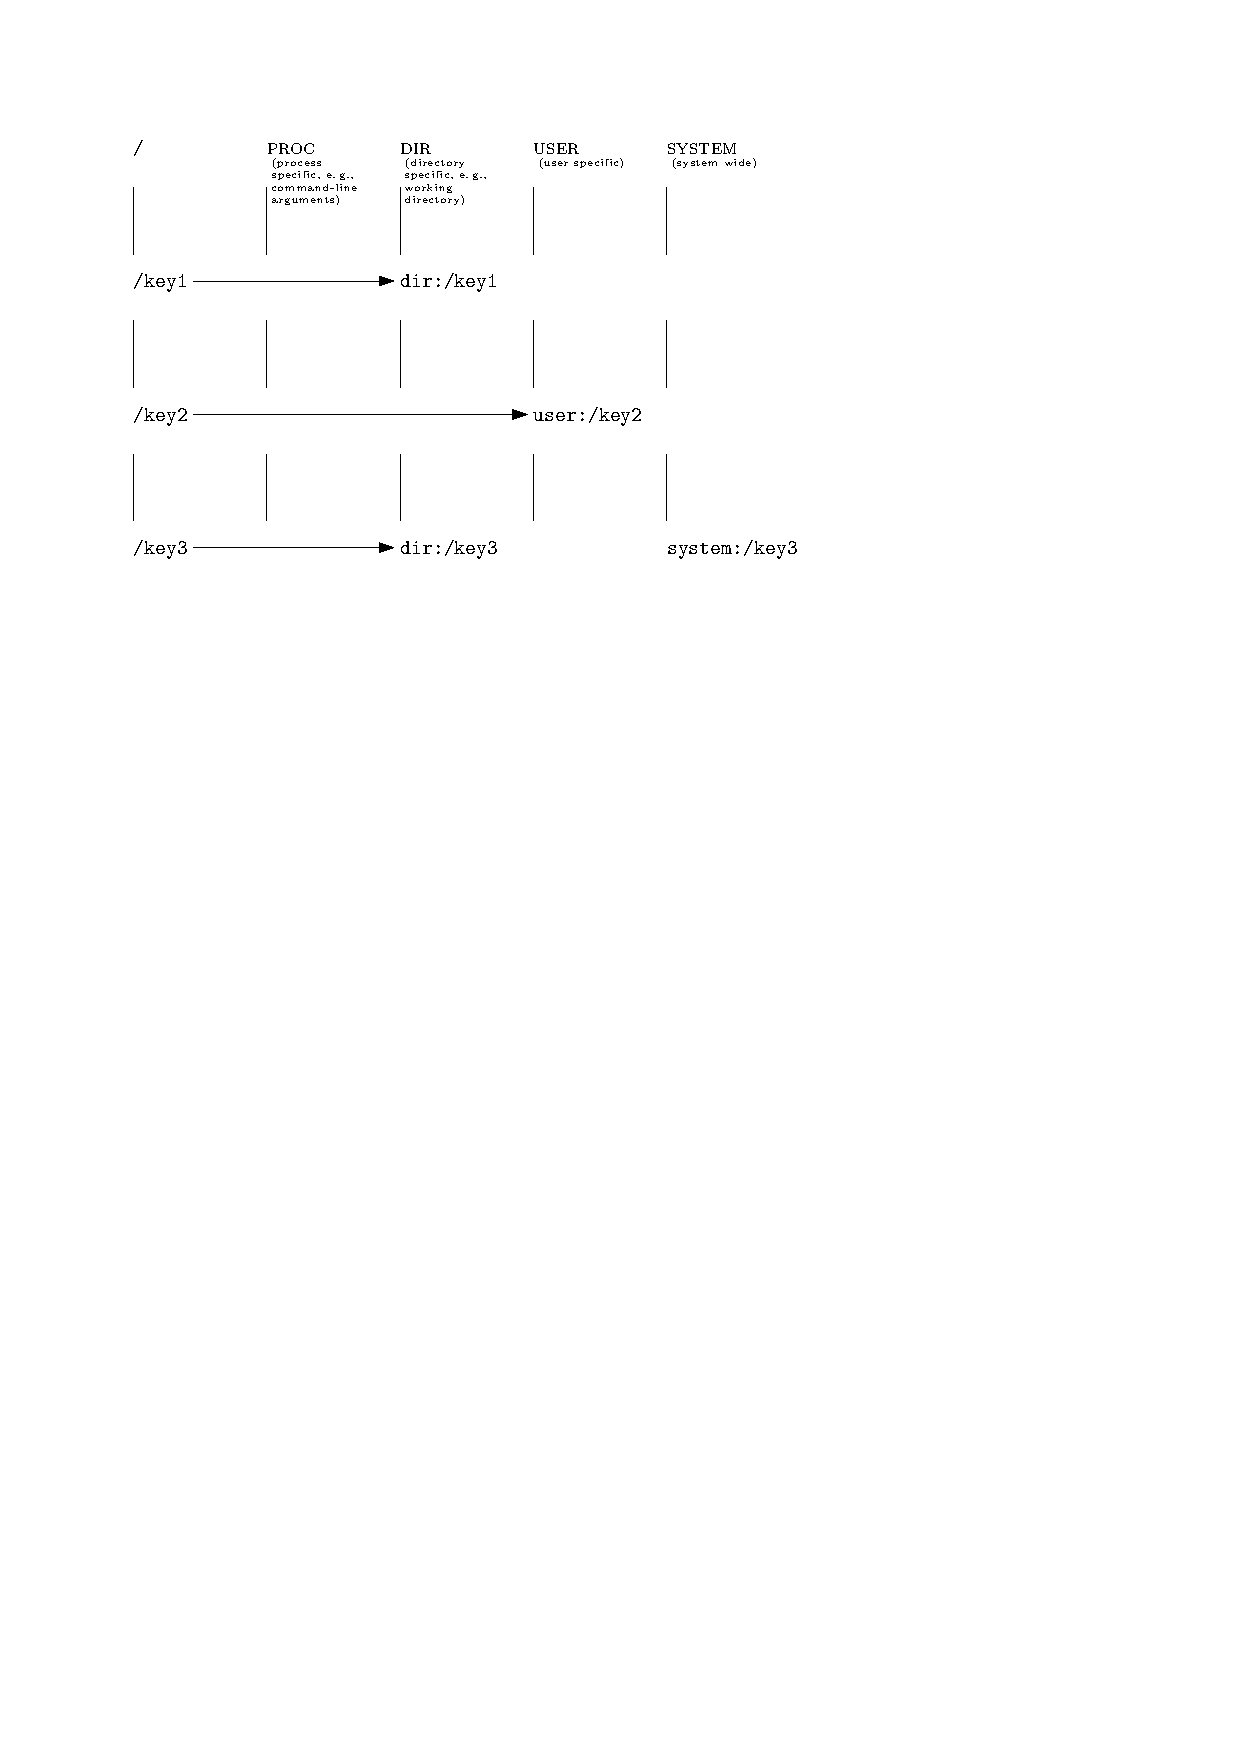
\includegraphics{cascading}
\end{frame}

\begin{frame}
	\frametitle{Context-oriented Programming}
	\ExecuteMetaData[../book/background.tex]{context-oriented-programming}
\end{frame}

\begin{frame}
	\frametitle{Contextual Values}
	\ExecuteMetaData[../book/background.tex]{contextual-values}
\end{frame}

\begin{frame}[fragile]
	\frametitle{Contextual Values (Pseudocode)}

	\begin{code}[gobble=4,language=C++,morekeywords={context}]
	void printBrowserConfig (Config config)
	{
		context.with("private")
		{
			println (config.keepHistory);
		}
		// same thread, different context:
		println (config.keepHistory);

		context.activate(currentLocation)
	}
	\end{code}
\end{frame}
\begin{frame}
	\frametitle{Introspection vs. Code Generation (Partly Recapitulation)}

	Implementation of contextual values might be in key database or in generated code.
	Advantages/Disadvantages?

	\pause

	\setbeamersize{description width=1cm}
	\begin{description} %[leftmargin=0cm] %TODO: move left
	\item[$-$] more techniques for performance improvements with code generation
	\item[$+$] specification can be updated live on the system without recompilation
	\item[$+$] tooling has generic access to all specifications
 	\item[$+$] new features the key database (e.g., better validation) are immediately available consistently
	\item[$-$] \color{red} needed if context differs within same thread
	\end{description}

	\vspace{0.5em}

	\begin{alertblock}{Implication}
	We generally prefer introspection, except for a very thin configuration access API.
	\end{alertblock}
\end{frame}


\begin{assignment}
	\begin{task}
	Break.
	\end{task}
\end{assignment}

\begin{frame}[fragile]
	\frametitle{Context Specifications (Recapitulation)}

	\begin{itemize}
	\item
	Determine threads from CPUs:

	\begin{code}[gobble=4]
	[env/layer/cpu]
	  type:=long
	[slapd/threads/listener]
	  context:=/slapd/threads/%cpu%/listener
	\end{code}

	\item
	Determine vibration from sensors:

	\begin{code}[gobble=4]
	[phone/call/vibration]
	  type:=boolean
	  context:=/phone/call/%inpocket%/vibration
	\end{code}

	\item
	Determine proxy settings from network:

	\begin{code}[gobble=4]
	[env/override/http_proxy]
	  context:=/http_proxy/%interface%/%network%
	\end{code}
	\end{itemize}
\end{frame}


\begin{frame}
	\frametitle{Types of Specifications (Recapitulation)}
	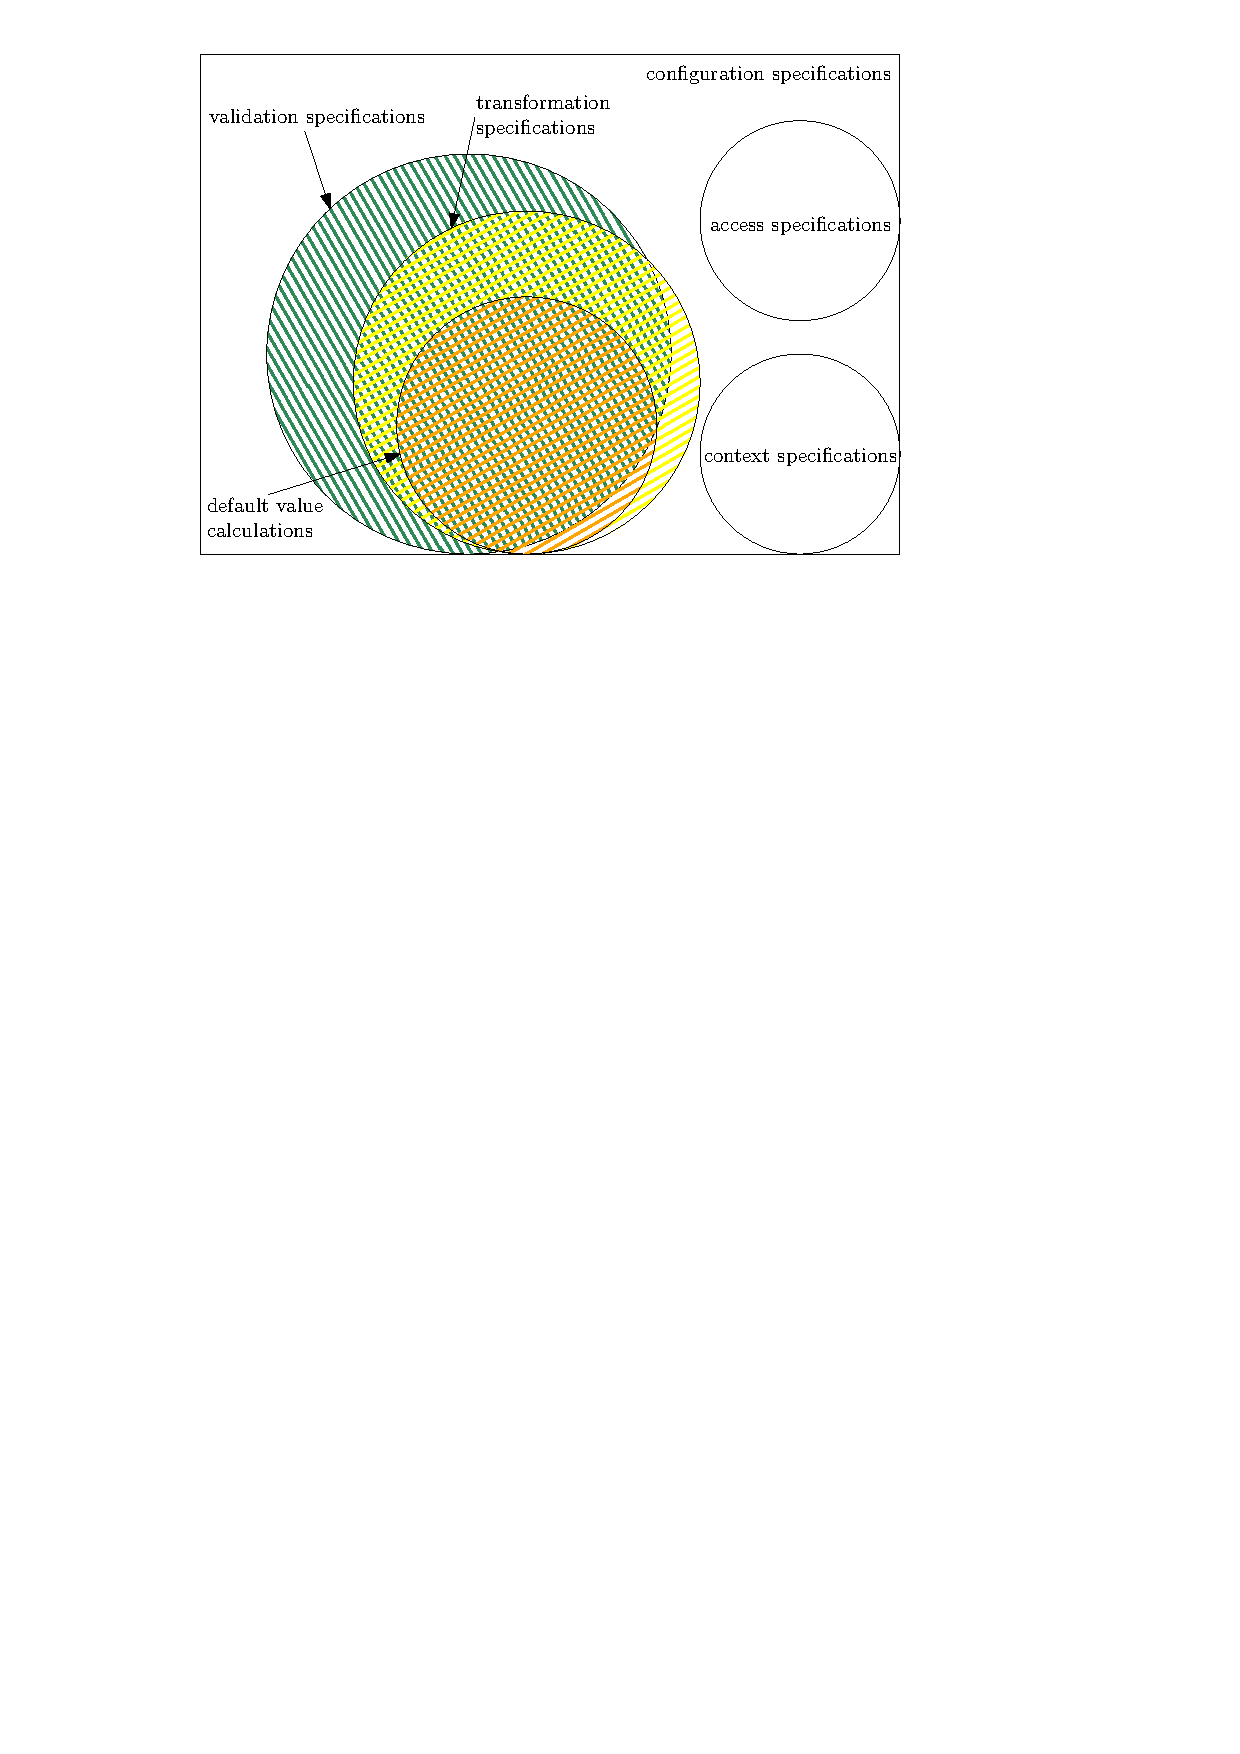
\includegraphics[scale=0.8]{specifications}
\end{frame}


%%%%%%%%%%%%%%%%%%%%%%%%%%%%%%%%%%%%%%%%%% 
\section{Key Databases}

\subsection{}

\begin{frame}
	\frametitle{Status Quo}

	Applications \dots

	\begin{itemize}
	\item usually consume configuration settings from configuration files, command-line arguments, and environment variables.
	\item sometimes have a single GUI or CLI for configuration settings.
	\item rarely have an API to access configuration settings.
	\item rarely consider context.
	\item rarely do in-depth validation.
	\item nearly never have an API to access configuration specifications.
	\end{itemize}

	\begin{task}
	Think about applications you know.
	Discuss it with your neighbor.
	\end{task}
\end{frame}

\begin{frame}
	\frametitle{Examples}

	\begin{itemize}
	\item Postfix\footnote{\url{http://www.postfix.org/OVERVIEW.html}}: CLI (Properties, CSV, and others)
	\item KDE\footnote{\url{https://api.kde.org/frameworks/kconfig/html/}}: GUI, CLI (INI)
	\item Libreoffice: GUI (XML)
	\item Firefox~\cite{jin2014configurations}: GUI (JavaScript and others)
	\item sudo: CLI (sudoers edited with visudo)
	\item X.org\footnote{\url{ftp://www.x.org/pub/X11R6.7.0/doc/xorg.conf.5.html}}: xorg.conf
	\item gpsd\footnote{\url{http://www.aosabook.org/en/gpsd.html}}: environment variables and command-line arguments
	\end{itemize}
\end{frame}

\begin{frame}
	\frametitle{Decisions}

	There are many ways to design configuration access but many decisions are only pragmatic and irrelevant with proper key/value abstraction.

	\begin{task}
	Which decisions are there?
	Why are they (ir)relevant?
	\end{task}

	\pause

	\begin{itemize}
	\item Which configuration file format? (irrelevant due to key/values)
	\item Split up into multiple configuration files? (irrelevant due to 3-way merging)
	\item Where are the configuration files? (irrelevant due to mounting and resolver)
	\item Important: Introspection, Validation, Horizontal Modularity, Integration,
		Specification, API, Guarantees, \dots
	\end{itemize}
\end{frame}

\begin{frame}
	\frametitle{Key Databases (Usage)}

	\methodQuestion{} \question{Which configuration systems/libraries/APIs have you already used or would like to use in one of your FLOSS project(s)?}

	\begin{itemize}
	\item Command-line arguments (\p{92}, $n=222$)
	\item environment variables (\p{79}, $n=218$)
	\item configuration files (\p{74}, $n=218$)
	\item Freedesktop standards (\p{20}, $n=205$)
	\item Windows Registry (\p{13}) ($\leq$ \p{13}, $n\geq185$) [talk later]
	\item X/Q/GSettings (\p{4}, \p{11}, \p{9})
	\item KConfig (\p{5})
	\item dconf (\p{7})
	\item plist (\p{7})
	\end{itemize}

\end{frame}

\begin{frame}
	\frametitle{Distributed Key Databases}

	Examples:

	\begin{itemize}
	\item Redis: in-memory with persistence and notification
	\item Zookeeper
	\item etcd:
		\begin{itemize}
		\item not in-memory
		\item get/set/watch interface via REST
		\item distributed coordination~\cite{ongaro2014search}
		\item needs configuration itself
		\end{itemize}
	\item Kubernetes: ConfigMaps
	\end{itemize}
\end{frame}

\begin{frame}
	\frametitle{}
	Many applications require configuration via some combination of config files, command line arguments, and environment variables. These configuration artifacts should be decoupled from image content in order to keep containerized applications portable. The ConfigMap API resource provides mechanisms to inject containers with configuration data while keeping containers agnostic of Kubernetes. ConfigMap can be used to store fine-grained information like individual properties or coarse-grained information like entire config files or JSON blobs.
	\par\raggedleft--- \textup{Kubernetes ConfigMaps}
\end{frame}

\begin{frame}
	\frametitle{Elektra}

	\begin{itemize}
	\item is not only a key database but a specification language to describe a key database
	\item plugins implement the specification (could be distributed but focus is configuration files)
	\item is library based (no single point of failure, no distributed coordination needed)
	\item supports transactions (persisting whole KeySets at once)
	\item supports integration of existing configuration
	\end{itemize}
\end{frame}



%%%%%%%%%%%%%%%%%%%%%%%%%%%%%%%%%%%%%%%%%% 
\section{History of Configuration Management}

\begin{frame}
	\frametitle{Definition}

	\intro[configuration management]{Configuration Management}:

	\begin{itemize}
	\item is a discipline in which configuration (in the broader sense) is administered.
	\item makes sure computers are assembled from desired parts and the correct applications are installed.
	\item ensures that the execution environment of installed applications is as required.%
	\end{itemize}
\end{frame}


\begin{frame}
	\frametitle{Definition}

	\intro[configuration management tool]{Configuration management tools}:

	\pause

	\begin{itemize}
	\item help people involved in configuration management.
	\item have means to describe the desired configuration of the whole managed system.
	\item try to converge the actual configuration to the desired one~\cite{burgess1995cfengine}.
	\end{itemize}
\end{frame}


\begin{frame}
	\frametitle{}

	Challenging tasks in configuration management:

	\pause

	\begin{itemize}
	\item inventory list
	\item installing packages
	\item monitoring
	\item add/replace machines
	\item maintaining files/databases/\dots
	\item \intro{configuration file manipulation}
	\end{itemize}
\end{frame}

%TODO: add more examples!


\begin{frame}
	\frametitle{Cloning}

	It all started with:

	\begin{itemize}
	\item clone all files with dd, rdist, rsync or unison (``golden image'')
	\item then do necessary modifications with scripts or profiles
	\end{itemize}

	\pause
	\vspace{3em}
	\hspace{-3em}

	\setbeamersize{description width=1cm}
	\begin{description} %[leftmargin=0cm] %TODO: move left?
	\item[$+$] works very good for many identical stateless machines
	\item[$-$] fails if differences between machines are too big
	\end{description}
\end{frame}

\begin{frame}
	\frametitle{Scripts}

	First improvement: have a script to create the ``golden image''.
	Possible benefits:

	\begin{itemize}[<+-| alert@+>]
	\item Documentation
	\item Customization (using configuration settings)
	\item \textbf{Reproducability}: Reproduce creation using different operating system versions
	\end{itemize}
\end{frame}

\begin{frame}[fragile]
	\frametitle{Profiles}

	\intro[profile]{Profiles} are groups of configuration settings between which the user can easily switch.

	\begin{itemize}
	\item by hostname, information EEPROM, manual selection, \dots
	\item can be activated as context:
	\end{itemize}

	\begin{code}[morekeywords={long},gobble=4]]
	[%application%/profile]
	  type:=string
	  opt:=p
	  opt/long:=profile
	  default:=
	\end{code}
\end{frame}


\begin{frame}
	\frametitle{First four configuration management tools}
	Cloning, and then NIS/NFS, was state of the art for a long time, until in 1994 when \enquote{the community nearly exploded with four new configuration systems}~\cite{evard1997analysis}:

	\ExecuteMetaData[../book/background.tex]{configuration-management-first-four}
\end{frame}

\begin{frame}
	\frametitle{Possible Benefits}

	\begin{itemize}[<+-| alert@+>]
	\item All advantages scripts have: \\
		Documentation, Customization, Reproducability
	\item Declarative description of the system \\
		(Infrastructure as Code~\cite{waldemar2013testing})
	\item Auditability
	\item Less configuration drift
	\item Error handling
	\item Pull/Push
	\item Reusability
	\item (Resource) Abstractions
	\end{itemize}
\end{frame}


\begin{frame}
	\frametitle{Conclusion and Outlook}

	\begin{itemize}[<+-| alert@+>]
	\item Context-awareness is a goal.
	\item Contextual values is a way to implement it.
	\item Many (distributed) key databases enable us to persist configuration settings.
	\item Definition and challenges in configuration management.
	\item Cloning: There and back again.
	\end{itemize}
\end{frame}






%%%%%%%%%%%%%%%%%%%%%%%%%%%%%%%%%%%%%%%%%% 
\nocite{raab2017introducing}

\appendix

\begin{frame}[allowframebreaks]
	\bibliographystyle{plainnat}
	\bibliography{../shared/elektra.bib}
\end{frame}

\end{document}


%TODO: add cliffhanger with preview for next time
